%-*-latex-*-
\sectionthree{Random variable}
\begin{python0}
from solutions import *; clear()
\end{python0}

Now for the definition of a very confusing term: random variable.
A \defone{random variable} $X$ of $S$ (a sample space) is just a function
from $S$ to some set, say $V$.
\[
  X : S \rightarrow V
\]
Usually $V$ is the set of real numbers:
\[
  X : S \rightarrow \R
\]
It's really important to remember that a random variable
is not random and is not a variable!!!
It's just a function from a sample space to a set.
This is an example of a badly chosen name for this idea.

There are two main reasons why we need the concept of random variables.
Pay attention to the following.



\newpage
\subsection{Random variable as labels}

The first reason for having random variables is
that we want to create some 
labels for the values in a sample space.
The labels will then create subsets of the sample space, i.e.,
random variables helps create meaningful events.

As an example, I'm going back to the die roll experiment.
The sample space is
\[
S = \{\ONE, \TWO, \THREE, \FOUR, \FIVE, \SIX \}
\]
Suppose I'm playing a game with a die and I win
if the roll gives me either $\ONE$ or $\SIX$;
otherwise I lose.
I can then define the following
random variables:
\[
  X : \{ \ONE, ..., \SIX \} \rightarrow \{ \GOOD, \BAD \}
\]
where
\begin{align*}
  X(\ONE) &= X(\SIX) = \textsc{Good} \\
  X(\TWO) &= X(\THREE) = X(\FOUR) = X(\FIVE) = \BAD 
\end{align*}
We have create two subsets
\begin{align*}
  A &= \{ s \in S \mid X(s) = \GOOD \} \\
  B &= \{ s \in S \mid X(s) = \BAD \}
\end{align*}
of $S$.
In other words, random variables create events for each
value in the range of the random variables.
In fact the subsets created are disjoint
and the union of all these subsets for the original
sample space.
In other words, $X$ creates a partition of the sample space,
i.e., $A$ and $B$ are disjoint and $A \cup B$ is $X$.

As a consequence, my random variable $X$ also defines a new
probability distribution function
\[
  p_X : \{ \GOOD, \BAD \} \rightarrow [0,1]
\]
where
\begin{align*}
  p_X(\GOOD) &= p(\{ s \in S \mid X(s) = \GOOD \}) = 1/3 \\
  p_X(\BAD) &= p(\{ s \in S \mid X(s) = \BAD \}) = 2/3
\end{align*}
This function is very frequently written like this:
\begin{align*}
  \Pr[X = \GOOD] &= 1/3 \\
  \Pr[X = \BAD] &= 2/3
\end{align*}
or sometimes
$\operatorname{P}[X=\GOOD]$
or
$\operatorname{P}(X=\GOOD)$.
This $\Pr$ is a bad notation because this function
actually depends on $p$ and $X$.
But nobody write $\Pr_p[X = \GOOD]$.
Part of the reason is because a random variable $X$
is usually tied to a probability distribution function.
Which is not exactly true since $X$ is a function of
the sample space and is therefore tied to the sample space
and not the probability function itself.
But this is the practice and you have to remember what I said
above in order not to be confused.

It's important to note that $p_X$ and $\Pr[X= \bullet]$ are pdfs,
but they are \textit{not} pdf on $S$: they are pdfs on
$\{ \GOOD, \BAD \}$.

Here's a picture to keep in mind:
\begin{center}

\begin{tikzpicture}

\draw (6.0, 1.0)
  node[draw, , , color=black,
       rounded corners=0cm, inner sep=0cm] {

\begin{minipage}[t][2cm]{12cm}
\mbox{}

\end{minipage}

};
\draw (0.5, 1.0)
  node[fill=blue!20!white,rounded corners=0cm,inner sep=0cm] {

\begin{minipage}[t][2cm]{1cm}
\mbox{}

\end{minipage}

};
\draw (0.5, 1.0)
  node[draw, , , color=black,
       rounded corners=0cm, inner sep=0cm] {

\begin{minipage}[t][2cm]{1cm}
\mbox{}

\end{minipage}

};
\draw (6.5, 0.25)
  node[draw=none, line width=0cm, , color=black,
       rounded corners=0cm, inner sep=0cm] {

\begin{minipage}[t][0.1cm]{0.1cm}
\mbox{}

\end{minipage}

};\draw (6.5, 0.25) node[color=black] {$n - 1$};
\end{tikzpicture}

\end{center}



The function at the top is $p$ and the function
at the bottom is $\Pr[X = \bullet]$.
You can (and should) think of a random variable as
collecting probabilities given by $p$ into buckets.
You can think of it this way:

\begin{center}
\begin{tikzpicture}

\fill[blue!10] (0.0, 0.0) circle (0.3);
\node [line width=0.03cm,black,minimum size=0.57cm,draw,circle] at (0.0,0.0)(a){};\draw (0.0, 0.0) node[color=black] {$a$};
\fill[blue!10] (-2.0, -1.0) circle (0.3);
\node [line width=0.03cm,black,minimum size=0.57cm,draw,circle] at (-2.0,-1.0)(b){};\draw (-2.0, -1.0) node[color=black] {$b$};
\fill[blue!10] (2.0, -1.0) circle (0.3);
\node [line width=0.03cm,black,minimum size=0.57cm,draw,circle] at (2.0,-1.0)(d){};\draw (2.0, -1.0) node[color=black] {$d$};
\fill[blue!10] (-3.0, -2.0) circle (0.3);
\node [line width=0.03cm,black,minimum size=0.57cm,draw,circle] at (-3.0,-2.0)(e){};\draw (-3.0, -2.0) node[color=black] {$e$};
\fill[blue!10] (-1.0, -2.0) circle (0.3);
\node [line width=0.03cm,black,minimum size=0.57cm,draw,circle] at (-1.0,-2.0)(f){};\draw (-1.0, -2.0) node[color=black] {$f$};
\fill[blue!10] (1.0, -2.0) circle (0.3);
\node [line width=0.03cm,black,minimum size=0.57cm,draw,circle] at (1.0,-2.0)(h){};\draw (1.0, -2.0) node[color=black] {$h$};
\fill[blue!10] (3.0, -2.0) circle (0.3);
\node [line width=0.03cm,black,minimum size=0.57cm,draw,circle] at (3.0,-2.0)(o){};\draw (3.0, -2.0) node[color=black] {$o$};
\fill[blue!10] (-2.5, -3.0) circle (0.3);
\node [line width=0.03cm,black,minimum size=0.57cm,draw,circle] at (-2.5,-3.0)(l){};\draw (-2.5, -3.0) node[color=black] {$l$};
\fill[blue!10] (1.5, -3.0) circle (0.3);
\node [line width=0.03cm,black,minimum size=0.57cm,draw,circle] at (1.5,-3.0)(m){};\draw (1.5, -3.0) node[color=black] {$m$};
\fill[blue!10] (3.5, -3.0) circle (0.3);
\node [line width=0.03cm,black,minimum size=0.57cm,draw,circle] at (3.5,-3.0)(j){};\draw (3.5, -3.0) node[color=black] {$j$};\draw[line width=0.03cm,black,->,>=triangle 60] (a) to  (b);
\draw[line width=0.03cm,black,->,>=triangle 60] (a) to  (d);
\draw[line width=0.03cm,black,->,>=triangle 60] (b) to  (e);
\draw[line width=0.03cm,black,->,>=triangle 60] (b) to  (f);
\draw[line width=0.03cm,black,->,>=triangle 60] (d) to  (h);
\draw[line width=0.03cm,black,->,>=triangle 60] (d) to  (o);
\draw[line width=0.03cm,black,->,>=triangle 60] (e) to  (l);
\draw[line width=0.03cm,black,->,>=triangle 60] (h) to  (m);
\draw[line width=0.03cm,black,->,>=triangle 60] (o) to  (j);
\end{tikzpicture}

\end{center}



The random variable $X$ basically collects up probabilities:
$\ONE$ and $\SIX$ are collected up into \GOOD\
and the rest are collected up into \BAD.

It's possible, in fact it's common, to have multiple
random variables on the same sample space.

Here's another random variable:
\[
Y : S \rightarrow \{ \EVEN, \ODD \}
\]
where
\begin{align*}
Y(\ONE) &= Y(\THREE) = Y(\FIVE) = \ODD \\
Y(\TWO) &= Y(\FOUR) = Y(\SIX) = \EVEN
\end{align*}
This means that we can talk about
\[
\Pr[Y = \ODD]
\]
which of course is just
\[
p(\{s \in S \mid Y(s) = \ODD \})
\]
Our $Y$ allows us to create the following subsets of $S$:
\begin{myenum}
  \li $\{ x \in S \mid Y(x) = \EVEN \} = \{\TWO, \FOUR, \SIX \} \subseteq S$
  \li $\{ x \in S \mid Y(x) = \ODD \} = \{\ONE, \THREE, \FIVE \} \subseteq S$
\end{myenum}
This $Y$ creates a pdf
\[
  \Pr[Y = \bullet] : \{ \EVEN, \ODD \} \rightarrow [0, 1]
\]
where
\[
  \Pr[Y = \EVEN] = \Pr[Y = \ODD] = \frac{1}{2}
\]

Here's yet another random variable on die rolls:
\[
Z : S \rightarrow \{ \textsc{Small}, \textsc{Medium}, \textsc{Large} \}
\]
where
\begin{align*}
Z(\ONE) &= Z(\TWO) = \textsc{Small} \\
Z(\THREE) &= Z(\FOUR) = \textsc{Medium} \\
Z(\FIVE) &= Z(\SIX) = \textsc{Large}
\end{align*}

Frequently instead of just
\[
  \Pr[Z = \textsc{Small}]
\]
you actually see expressions like this:
\[
  \Pr[Z = \textsc{Small} \text{ or } Z = \textsc{Medium}]
\]
or more formally
\[
  \Pr[Z \in \{\textsc{Small}, \textsc{Medium}\}]
\]
In other words
\[
  \Pr[\text{boolean expression on a random variable}]  
\]
and even boolean expressions involving more than one random variables:
\[
\Pr[Y = \ODD \lor Z = \text{Small}]  
\]
In this case
\[
\Pr[Y = \ODD \ \lor \ Z = \text{Small}]
=
\sum_{\stackrel{s \in S}{Y(s) = \ODD \ \lor \ Z(s) = \text{Small}}} p(s)
\]


Here's another random variable where the value of the random variable
takes a real values.
For instance, for the die rolling experiment, suppose I define $W$
in the obvious way:
\begin{align*}
W(\ONE) &= 1 \\
W(\TWO) &= 2 \\
W(\THREE) &= 3 \\
W(\FOUR) &= 4 \\
W(\FIVE) &= 5 \\
W(\SIX) &= 6 \\
\end{align*}
With this random variable $W$, I can write
\[
\Pr[W \text{ is odd}]
\]
to mean
$\Pr[W \in \{\ONE, \THREE, \FIVE\}]$.
I can even write
$\Pr[W \leq 4]$.
The meaning should be obvious.

In general, suppose $p : S \rightarrow \R$ is a probability distribution function
and $X : S \rightarrow V$ is a random variable.
If $v \in V$.
I will write $\Pr[X = v]$ for the following: 
\[
\Pr[X = v] = p(\{s \in S \mid X(s) = v \}) = p(X^{-1}(v))
\]
This function
\[
  \Pr[X = \bullet] : V \rightarrow [0, 1]
\]
is a pdf.
In other words, you can get a pdf from a pdf and a random variable $X$.

\textsc{WARNING}: In some books, instead of 
\begin{itemize}
\li \textsl{Let $p$ be the probability function
of tossing a coin that is twice as likely to get a head than a tail,
then
\[
p : \{\HEAD, \TAIL\} \rightarrow [0,1] 
\]
\[
p(\HEAD) = \frac{2}{3}, \,\,\,\,\,
p(\TAIL) = \frac{1}{3}"
\]
}
\end{itemize}
you might hear this:
\begin{itemize}
\li \textsl{Let $X$ be the random variable of tossing a coin 
that is twice as likely to get a head than a tail, then
\[
\Pr[X = \HEAD] = \frac{2}{3}, \,\,\,\,\,
\Pr[X = \TAIL] = \frac{1}{3}
\]
}
\end{itemize}
Treat them as the same.
Some authors do not differentiate between probability distribution
function and the probability distribution derived from a
random variable.
This practice is very common, so you have to learn to live with it.



\newpage
\subsection{Random variable as a scoring function; expectation}

Let $p: S \rightarrow [0,1]$ be a pdf.
Besides labels,
you can also think of the random variable $X$ on $S$
as some kind of 
\textit{scoring}
for each outcome of the sample space of an experiment:
\[
  X : S \rightarrow \R
\]
With this setup, 
we can define the 
average value or the
\defone{expected value} of $X$,
or the \defone{expectation} of $X$,
to be
\[
\E[X] = \sum_{s \in S} X(s) \cdot p(s)
\]
In this case,
$\E[X]$ is the average score you will get if you keep
drawing some outcome from $S$.
What I mean is this:

Suppose you close your eyes and randomly draw an $s_0$ from $S$
and note down the score of $s_0$, i.e., $X(s_0)$.
You put then $s_0$ back into $S$.
You repeat the above and get $s_1 \in S$
and note down the score $X(s_1)$.
You put $s_1$ back into $S$.
The average so far is $(X(s_0) + X(s_1))/2$.
You repeat the above and get $s_2 \in S$.
The average is now $(X(s_0) + X(s_1) + X(s_2))/3$.
You keep on going and you'll get the
theoretical average.
(\lq\lq Theoretical" because obviously you can't go on forever.)
The value of $\E[X]$ gives you this theoretical average.

Instead of summing over $X$, it's also possible to sum over all the possible
values of $X$:
\[
\E[X] = \sum_{x \in X(S)} x \cdot \Pr[X = x]
\]
See example below if you don't see why.
Here, $X(S)$ is the range of $X$, i.e.,
\[
  X(S) = \{X(s) \mid s \in S \}
\]

In many cases, the probability of an experiment is not what you're after.
It's usually some kind of \lq\lq gain''
or \lq\lq value"
from doing an experiment or playing a
probabilistic game -- which turns out to be the expectation of some
random variable.
This is what I mean:

Take a look at our random variable $X$:
\[
  X : \{ \ONE, ..., \SIX \} \rightarrow \{ \textsc{Good}, \textsc{Bad} \}
\]
where
\begin{align*}
  X(\ONE) &= X(\SIX) = \textsc{Good} \\
  X(\TWO) &= X(\THREE) = X(\FOUR) = X(\FIVE) = \textsc{Bad} 
\end{align*}
Suppose I now define another random variable:
\[
  X' : \{ \ONE, ..., \SIX \} \rightarrow \R
\]
\begin{align*}
  X'(\ONE) &= X'(\SIX) = 3 \\
  X'(\TWO) &= X'(\THREE) = X'(\FOUR) = X'(\FIVE) = -1 
\end{align*}
This could be for instance a gambing game where I get \$3
if I roll a one or a six; otherwise I lose \$1.
The expectation of $X'$ is
\[
  \E[X'] = \sum_{s \in S} X'(s) p(x)
\]
which is
\begin{align*}
  \E[X']
  &=
    X'(\ONE) p(\ONE)
    +X'(\TWO) p(\TWO)
    +X'(\THREE) p(\THREE)
  \\
  &\hspace{0.5cm}
    +X'(\FOUR) p(\FOUR)
    +X'(\FIVE) p(\FIVE)
    +X'(\SIX) p(\SIX)
  \\
  &=
         3 \cdot \frac{1}{6}
    + (-1) \cdot \frac{1}{6} 
    + (-1) \cdot \frac{1}{6}
    + (-1) \cdot \frac{1}{6} 
    + (-1) \cdot \frac{1}{6} 
    + 3    \cdot \frac{1}{6}
  \\
  &= \frac{1}{3}
\end{align*}
which tells me on the average I'm going to gain \$1/3 dollars, about 33 cents, per game.


Note that I can also calculate the probability distribution from $X'$:
\[
  \Pr: \{3, -1\} \rightarrow [0,1]
\]
to get
\begin{align*}
  \Pr[X' = 3] &= p(\{\ONE, \SIX \}) = 1/3 \\
  \Pr[X' = -1] &= p(\{ \TWO, \THREE, \FOUR, \FIVE \}) = 2/3 
\end{align*}
and then compute $\E[X']$ this way:
\begin{align*}
  \E[X']
  &= \sum_{x \in X'(S)} x \cdot \Pr[X' = x]
    \\
  &= 3 \cdot \Pr[X' = 3]
    + (-1) \cdot \Pr[X' = -1]
  \\
  &= 3 \cdot \frac{1}{3} + (-1) \frac{2}{3}
  \\
  &= \frac{1}{3}
\end{align*}
In general, if $X$ is a random variable with values in $\R$, then
\[
  \E[X] = \sum_{s \in S} X(s) \cdot p(x) = \sum_{x \in X(S)} x \cdot \Pr[X = x] 
\]

Suppose for this gambling game, to play the game, you have to pay \$0.5 (fifty cents)
for each roll.
You can work out $\E[X'] = 1/3$ and then subtract $0.5$ to get your gain per game
to get a gain of
\[
  \frac{1}{3} - 0.5 = -\frac{1}{6}
\]
Another way to do that is to include the cost of playing the game in the expectation
computation.
For instance you can define a random variable
\[
  Y' : \{\ONE, \TWO, \THREE, \FOUR, \FIVE, \SIX \} \rightarrow \R 
\]
as
\[
  Y'(s) = -0.5
\]
Then the gain from playing this game (including the cost of playing the game is
\[
  \E[X' + Y']
\]
where $X' + Y'$ is the random variable
\[
  X' + Y': \{\ONE, \TWO, \THREE, \FOUR, \FIVE, \SIX\} \rightarrow \R
\]
given by
\[
  (X' + Y')(s) = X'(s) + Y'(s)
\]
If you compute $\E[X' + Y']$ using $\E[X' + Y'] = \sum_{s \in S} (X(s) + Y(s)) p(s)$, you will get
\[
  (3 - 0.5) \frac{1}{6}
  + (-1 - 0.5) \frac{1}{6}
  + (-1 - 0.5) \frac{1}{6}
  + (-1 - 0.5) \frac{1}{6}
  + (-1 - 0.5) \frac{1}{6}
  + (3 - 0.5) \frac{1}{6}
  = -\frac{1}{6}
\]
If I use $\E[X' + Y'] = \sum_{z \in (X+Y)(S)} z \cdot \Pr[X+Y=z]$.
For this I'll need to know the range of $X + Y$:
\[
  (X + Y)(S) = \{3 - 0.5, -1 - 0.5\} = \{2.5, -1.5\} = \{2.5, -1.5\}
\]
and the probability distribution function of $\Pr[X + Y = \bullet]$ is
\begin{align*}
  \Pr[X + Y = 2.5]
  &= \{s \in S \mid (X + Y)(s) = 2.5\} \\
  &= p(\{ \ONE, \SIX \}) \\
  &= \frac{2}{6} = \frac{1}{3}
  \\
  \Pr[X + Y = -1.5]
  &= \{s \in S \mid (X + Y)(s) = -1.5\} \\
  &= p(\{\TWO, \THREE, \FOUR, \FIVE\}) \\
  &= \frac{4}{6} = \frac{2}{3}
\end{align*}
Therefore
\begin{align*}
  \E[X' + Y']
  &= \sum_{z \in (X'+Y')(S)} z \cdot \Pr[X'+Y'=z] \\
  &= 2.5 \cdot \frac{1}{3} + (-1.5) \cdot \frac{2}{3} \\
  &= -\frac{1}{6} 
\end{align*}
You can also use the formula
\[
  \E[X' + Y'] = \E[X'] + \E[Y']
\]
I already know that $\E[X'] = 1/3$.
$\E[Y']$ is easy:
\[
  \E[Y'] = (-0.5) \frac{1}{6} + \cdots + (-0.5) \frac{1}{6} = (-0.5)(1) = -0.5 
\]
Therefore $\E[X' + Y'] = 1/3 - 0.5 = -1/6$.

This is important:
Look at the three ways of computing
$\E[X' + Y']$ again.
Which is easier?
And, more importantly, why is the one that you picked
the easiest?

You'll find that computing $\E[X' + Y']$ using
\[
  \E[X' + Y'] = \E[X'] + \E[Y']
\]
is frequently the easiest.

In general if $X$ and $Y$ are random values:
\begin{align*}
X &: S \rightarrow \R \\
Y &: S \rightarrow \R
\end{align*}
then of course you can also consider
\[
X + Y : S \rightarrow \R
\]
This is clearly also a random variable.
Remember that random variables are just functions.
More generally, if there are $n$ random variables
\[
  X_i : S \rightarrow \R
\]
for $i = 0, 1, 2, \ldots, n - 1$,
then
\[
\sum_{i=0}^{n-1} X_i : S \rightarrow \R
\]
where
\[
\left( \sum_{i=0}^{n-1} X_i \right)(s)
=
\sum_{i=0}^{n-1} X_i(s)
\]
is also a random variable.
Furthermore 
\[
\E \left[ \sum_{i=0}^{n-1} X_i \right]
=
\sum_{i=0}^{n-1} \E \left[ X_i \right]
\]

At this point, it should not be surprising that
if I change the rules of the above gambling game so that
the random variable is $X'' = 2X'$, i.e.,
if you roll a one or a six you win $2 \cdot 3$ dollar
otherwise you lose $2 \cdot 1$ dollars, then
the average gain per game should be
\[
  \E[X''] = \E[2X'] = 2 \cdot \E[X']
\]
Right?

In general, if $a$ is a real number and $X:S \rightarrow \R$
is a random variable, then $aX: \rightarrow \R$ given by
\[
  (aX)(s) = a \cdot X(s)
\]
is also a random variable and furthermore
\[
  \E[aX] = a \cdot \E[X]
\]

%-*-latex-*-

\begin{ex} 
  \label{ex:prob-00}
  \tinysidebar{\debug{exercises/{disc-prob-28/question.tex}}}

  \solutionlink{sol:prob-00}
  \qed
\end{ex} 
\begin{python0}
from solutions import *
add(label="ex:prob-00",
    srcfilename='exercises/discrete-probability/prob-00/answer.tex') 
\end{python0}


It's also common to view a real number, say $b$, as a random variable.
What I mean is this random variable:
\[
  b : S \rightarrow \R
\]
where
\[
b(s) = b
\]
for any outcome $s$ in $S$.
In other words, I'm consider $b$ as a constant function.
For instance our
\[
Y' : \{ \ONE, \TWO, \THREE, \FOUR, \FIVE, \SIX \}
\]
above where
\[
  Y'(s) = -0.5
\]
(i.e., you have to pay 50 cents for every roll) is such as example.
So instead of defining $Y'$ and then say
\[
  \E[X' + Y'] = -\frac{1}{6}
\]
I could have just said
\[
  \E[X' - 0.5] = \E[X'] + \E[-0.5] = \frac{1}{3} + (-0.5) = -\frac{1}{6}
\]
(i.e., $Y'$ is just the constant function $Y' = -0.5$.)
Easy right?


Let me collection the above together as a theorem:

\begin{thm}
  For $i = 0, 1, 2, ..., n - 1$, 
  let $X_i$ be a (real-valued) random variable and $c_i$ be a constant. Let $c$ be a constant (viewed as a constant random variable).
  Then
  \[
  \E\left[ \sum_{i = 0} c_i X_i \right]
  =
  \sum_{i = 0} c_i \E\left[ X_i \right]
  \]
  and
  \[
  \E[c] = c
  \]
\end{thm}

%-*-latex-*-

\begin{ex} 
  \label{ex:prob-00}
  \tinysidebar{\debug{exercises/{disc-prob-28/question.tex}}}

  \solutionlink{sol:prob-00}
  \qed
\end{ex} 
\begin{python0}
from solutions import *
add(label="ex:prob-00",
    srcfilename='exercises/discrete-probability/prob-00/answer.tex') 
\end{python0}

%-*-latex-*-

\begin{ex} 
  \label{ex:prob-00}
  \tinysidebar{\debug{exercises/{disc-prob-28/question.tex}}}

  \solutionlink{sol:prob-00}
  \qed
\end{ex} 
\begin{python0}
from solutions import *
add(label="ex:prob-00",
    srcfilename='exercises/discrete-probability/prob-00/answer.tex') 
\end{python0}





\begin{comment}
\newpage
XXXXX

You are at XYZ Casino, confident of your new found knowledge of
computing probabilties.
You approach one of the tables to check out the game.
Here's the rule of the game: You have to pay \$10 to play the game.
You throw two dice, one at a time.
If the first die gives you 6, you win and get \$40.
Otherwise, your second roll must be the same as your first in which 
case you also win but you get only \$20.
Otherwise you lose and get nothing.
This does not seem to be difficult.
You just need to simulate the dice roll and return the gain like this:
\includesourcenonumbers{discrete-probability/game1.py}

Of course this is only one game.
You need to simulate lots of games to determine your 
\lq\lq ultimate'' gain, i.e., your average gain:
\includesourcenonumbers{discrete-probability/game2.py}

You quickly run your program and get this:
XXX
\begin{center}
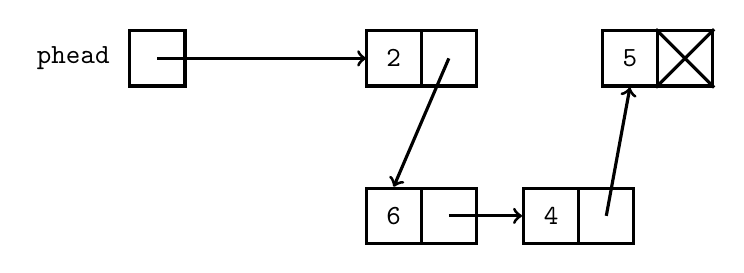
\begin{tikzpicture}

\draw (0.35, 0.35)
  node[draw, line width=0.04cm, , color=black,
       rounded corners=0cm, inner sep=0cm] {

\begin{minipage}[t][0.7cm]{0.7cm}
\mbox{}

\end{minipage}

};\draw (0.35, 0.35) node[color=black] {{\texttt{2}}};
\draw (1.0499999999999998, 0.35)
  node[draw, line width=0.04cm, , color=black,
       rounded corners=0cm, inner sep=0cm] {

\begin{minipage}[t][0.7cm]{0.7cm}
\mbox{}

\end{minipage}

};\draw (1.0499999999999998, 0.35) node[color=black] {{\texttt{}}};
\draw (0.35, -1.65)
  node[draw, line width=0.04cm, , color=black,
       rounded corners=0cm, inner sep=0cm] {

\begin{minipage}[t][0.7cm]{0.7cm}
\mbox{}

\end{minipage}

};\draw (0.35, -1.65) node[color=black] {{\texttt{6}}};
\draw (1.0499999999999998, -1.65)
  node[draw, line width=0.04cm, , color=black,
       rounded corners=0cm, inner sep=0cm] {

\begin{minipage}[t][0.7cm]{0.7cm}
\mbox{}

\end{minipage}

};\draw (1.0499999999999998, -1.65) node[color=black] {{\texttt{}}};
\draw (2.35, -1.65)
  node[draw, line width=0.04cm, , color=black,
       rounded corners=0cm, inner sep=0cm] {

\begin{minipage}[t][0.7cm]{0.7cm}
\mbox{}

\end{minipage}

};\draw (2.35, -1.65) node[color=black] {{\texttt{4}}};
\draw (3.0500000000000003, -1.65)
  node[draw, line width=0.04cm, , color=black,
       rounded corners=0cm, inner sep=0cm] {

\begin{minipage}[t][0.7cm]{0.7cm}
\mbox{}

\end{minipage}

};\draw (3.0500000000000003, -1.65) node[color=black] {{\texttt{}}};
\draw (3.35, 0.35)
  node[draw, line width=0.04cm, , color=black,
       rounded corners=0cm, inner sep=0cm] {

\begin{minipage}[t][0.7cm]{0.7cm}
\mbox{}

\end{minipage}

};\draw (3.35, 0.35) node[color=black] {{\texttt{5}}};
\draw (4.05, 0.35)
  node[draw, line width=0.04cm, , color=black,
       rounded corners=0cm, inner sep=0cm] {

\begin{minipage}[t][0.7cm]{0.7cm}
\mbox{}

\end{minipage}

};\draw (4.05, 0.35) node[color=black] {{\texttt{}}};\draw[line width=0.04cm,black,->] (1.05,0.35) to  (0.35,-1.28);
\draw[line width=0.04cm,black,->] (1.05,-1.65) to  (1.98,-1.65);
\draw[line width=0.04cm,black,->] (3.05,-1.65) to  (3.35,-0.02);
\draw[line width=0.04cm,black] (3.68,0.72) to  (4.42,-0.02);
\draw[line width=0.04cm,black] (4.42,0.72) to  (3.68,-0.02);

\draw (-2.65, 0.35)
  node[draw, line width=0.04cm, , color=black,
       rounded corners=0cm, inner sep=0cm] {

\begin{minipage}[t][0.7cm]{0.7cm}
\mbox{}

\end{minipage}

};\draw (-2.65, 0.35) node[color=black] {{\texttt{}}};\draw[line width=0.04cm,black,->] (-2.65,0.35) to  (0,0.35);

\draw (-3.7199999999999998, 0.35)
  node[draw, line width=0.04cm, , color=white,
       rounded corners=0cm, inner sep=0cm] {

\begin{minipage}[t][0.1cm]{0.1cm}
\mbox{}

\end{minipage}

};\draw (-3.7199999999999998, 0.35) node[color=black] {{\texttt{phead}}};
\end{tikzpicture}

\end{center}



YIKE!!!
You're going to lose!!!
What crooks!

OK ... let's go back to the math behind this game.
Immediately, you should ask this question:
How can you compute this gain quickly?
In particular, where does the probability function for a single die roll
\[
p(x) = \frac{1}{6} \hspace{1cm} 
\text{for $x \in \{\ONE, \TWO, \THREE, \FOUR, \FIVE, \SIX\}$}
\]
come in?
Can we compute the gain mathematically without a computer simulation?

To simplify the argument, suppose you roll one die and
it's free to play the game.
If the outcome is 1, I will give you \$0.
If the outcome is 2, you will give me \$1.
If the outcome is 3, I will give me \$2.
If the outcome is 4, you will give me \$3.
If the outcome is 5, I will give me \$4.
If the outcome is 6, you will give me \$5.
Suppose we play a total of 60 games, 
where there are 
10 outcomes of die value 1, 
15 outcomes of die value 2, 
11 outcomes of die value 3,
20 outcomes of die value 4, 
8 outcomes of value 5, and
18 outcomes of value 6.
What is the total gain for you?
It should be
\[
0 \cdot 10 + (-1) \cdot 15 + 2 \cdot 11 + (-3) \cdot 20 + 
4 \cdot 8 + (-5) \cdot 18 
\]
And your average gain per game is then
\[
\frac
{0 \cdot 10 + (-1) \cdot 15 + 2 \cdot 11 + (-3) \cdot 20 + 
4 \cdot 8 + (-5) \cdot 18}
{10 + 15 + 11 + 20 + 8 + 18}
\]
Let $n_\ONE = 10$ (i.e. number of times you get $\ONE$), 
$n_\TWO = 15$, $n_\THREE = 11$, $n_\FOUR = 20$, $n_\FIVE = 8$, 
and $n_\SIX = 18$.
Let $n = n_\ONE + n_\TWO + \cdots + n_\SIX$.
Then the above becomes:
\begin{align*}
&\frac
{0 \cdot 10 + (-1) \cdot 15 + 2 \cdot 11 + (-3) \cdot 20 + 
4 \cdot 8 + (-5) \cdot 18}
{10 + 15 + 11 + 20 + 8 + 18}
\\
&= 
\frac
{0 \cdot n_\ONE + (-1) \cdot n_\TWO + 2 \cdot n_\THREE + (-3) \cdot n_\FOUR + 
4 \cdot n_\FIVE + (-5) \cdot n_\SIX}
{n} \\
&= 
0 \cdot \frac{n_\ONE}{n} + 
(-1) \cdot \frac{n_\TWO}{n} + 
2 \cdot \frac{n_\THREE}{n} + 
(-3) \cdot \frac{n_\FOUR}{n} + 
4 \cdot \frac{n_\FIVE}{n} + 
(-5) \cdot \frac{n_\SIX}{n}
\end{align*}
Wait a minute ... $\frac{n_\ONE}{n}$ is the ratio of
outcomes which is $\ONE$. 
That's just the probability of getting 1 ...
well, if the number of experiments is large, i.e., when $n$ is large.
If we write $p(x)$ for the probability function of our die, we get:
\begin{align*}
&
0 \cdot \frac{n_\ONE}{n} + 
(-1) \cdot \frac{n_\ONE}{n} + 
2 \cdot \frac{n_\THREE}{n} + 
(-3) \cdot \frac{n_\FOUR}{n} + 
4 \cdot \frac{n_\FIVE}{n} + 
(-5) \cdot \frac{n_\SIX}{n}
\\
&= 
0 \cdot p(\ONE) + 
(-1) \cdot p(\TWO) + 
2 \cdot p(\THREE) + 
(-3) \cdot p(\FOUR) + 
4 \cdot p(\FIVE) + 
(-5) \cdot p(\SIX)
\end{align*}
For this game, if the die value is $\ONE$, your gain is 0,
if it's $\TWO$, your gain is -1, etc.
For the time being we write $X(x)$ for the gain for value $x$.
The above average gain becomes
\[
X(\ONE) p(\ONE) + \cdots X(\SIX) p(\SIX)
= \sum_{x \in S} X(x) p(x)
\]
where $S = \{\ONE, ..., \SIX\}$.
Now you say ... \lq\lq OK, great. Now I know how to gamble.
But what has this to do with computer science?!?''

One application of probability theory is the runtime computation
of algorithms.
For instance if you have the following 
\begin{Verbatim}[frame=single]
if (x == 0):
    f(x)
else:
    g(x)
\end{Verbatim}
Suppose for this pseudocode, there is s probability of 1/3 that $x$ is 0
and 2/3 if $x$ is 1.
(There are no other possible values for $x$.)
Furthermore, the time taken to execute \verb!f(0)! is $X(0)$ and 
the time taken to execute $g(1)$ is $X(1)$, then
the average time to execute this pseudocode is
\[
X(0) \cdot \frac{1}{3} + X(1) \cdot \frac{2}{3}
\]

Using this new idea, let's compute the average value of our
casino game.
First of all let's list the outcomes:
it's $(x, y)$ where $x$ and $y$ are outcomes of rolling dice.
The probability (assuming XYZ has not digged their dice) is
\[
p((x,y)) = \frac{1}{36}
\]
What about the random variable?
The first rule says
\[
X((6, y)) = 40 - 10 = 30
\]
for $y \in \{1,2,3,4,5,6\}$.
There are 6 such cases.
The second rule says that
\[
X((x,x)) = 20 - 10 = 10
\]
for $x \neq 6$.
There are 5 such cases.
For all other cases
\[
X((x,y)) = 0 - 10 = -10
\]
There are $36 - 6 - 5 = 25$ such cases.
Therefore your gain is
\begin{align*}
\E[X] 
&= \frac{1}{36}[6 \cdot 30 + 5 \cdot 10 + 25 \cdot (-10)]
  = \frac{1}{36}[180 + 50 - 250] \\
&= -\frac{20}{36} = -\frac{5}{9} \\
&\approx -0.5555
\end{align*}


Suppose now I toss two fair coins.
What is the probability of getting two heads?
When you're given a problem like the above, you can see quickly
that it must be 1/4 and that's because the problem is so simple.
However when the problem is more complicated, you cannot rely on your
intuition!
Let's rephrase the above with proper mathematical objects:
First you need a sample space $S$.
The outcomes are
\renewcommand\HEAD{\texttt{HEAD}}
\renewcommand\TAIL{\texttt{TAIL}}
\begin{tightlist}
\item First coin gives me a $\HEAD$, second gives me a $\HEAD$
\item First coin gives me a $\HEAD$, second gives me a $\TAIL$
\item First coin gives me a $\TAIL$, second gives me a $\HEAD$
\item First coin gives me a $\TAIL$, second gives me a $\TAIL$
\end{tightlist}
It would make me go crazy if I have to describe the events with
so many words.
So I'm going to use
\begin{tightlist}
\item $(\HEAD, \HEAD)$
\item $(\HEAD, \TAIL)$
\item $(\TAIL, \HEAD)$
\item $(\TAIL, \TAIL)$
\end{tightlist}
to denote the above outcomes.
Since the coins are fair, you would expect these four outcomes to be 
equally likely, i.e.,
the pdf 
\begin{align*}
p &: \{(\HEAD, \HEAD),
(\HEAD, \TAIL),
(\TAIL, \HEAD),
(\TAIL, \TAIL)\} 
\rightarrow [0,1]
\end{align*}
is given by 
\begin{align*}
p((\HEAD, \HEAD)) &= 1/4 \\
p((\HEAD, \TAIL)) &= 1/4 \\
p((\TAIL, \HEAD)) &= 1/4 \\
p((\TAIL, \TAIL))  &= 1/4 
\end{align*}
And of course, the probability of getting two heads is 
\[
p((\HEAD, \HEAD)) = 1/4
\]


You can think of $X$ as assigning some kind of gain in a probabilitistic
game. 
For instance in the case of tossing a rigged coin with
\[
p(\HEAD) = \frac{2}{3}, \,\,\,\,\,
p(\TAIL) = \frac{1}{3}
\]
suppose I play a game with you where I toss a coin and I want to count
the number of heads, I would set
\[
X(\HEAD) = 1, \,\,\,\,\,
X(\TAIL) = 0
\]
Or for instance suppose we play a game where if I toss my toss
and you see a head, then you give me \$2 and if you see a tail,
I will give you \$3.
In this case, we can define a random variable
\[
X(\HEAD) = -2, \,\,\,\,\,
X(\TAIL) = 3
\]
In this case, the random variable is your gain in playing the game.
(Will you play the game?)


[PUT THIS IN A DIFFERENT SECTION]
The variance of $X$ is
\[
\Var[X]
\]

\end{comment}





\newpage
\subsection{Labeling and scoring}

Frequently,
a random variable is used for both labeling and scoring.
For instance
\[
  X' : \{ \ONE, \TWO, \THREE, \FOUR, \FIVE, \SIX \} \rightarrow \R
\]
with
\begin{align*}
  X'(\ONE) &= X'(\SIX) = 3 \\
  X'(\TWO) &= X'(\THREE) = X'(\FOUR) = X'(\FIVE) = -1 
\end{align*}
$X'$ scores the outcomes, but $X'$ (obviously)
also label outcomes based on their scores.


%-*-latex-*-

\begin{ex} 
  \label{ex:prob-00}
  \tinysidebar{\debug{exercises/{disc-prob-28/question.tex}}}

  \solutionlink{sol:prob-00}
  \qed
\end{ex} 
\begin{python0}
from solutions import *
add(label="ex:prob-00",
    srcfilename='exercises/discrete-probability/prob-00/answer.tex') 
\end{python0}

%-*-latex-*-

\begin{ex} 
  \label{ex:prob-00}
  \tinysidebar{\debug{exercises/{disc-prob-28/question.tex}}}

  \solutionlink{sol:prob-00}
  \qed
\end{ex} 
\begin{python0}
from solutions import *
add(label="ex:prob-00",
    srcfilename='exercises/discrete-probability/prob-00/answer.tex') 
\end{python0}
 
